\begin{lstlisting}[frame=lines, style=Rust, caption={Simple Proof of Concept Wasm Serverless Platform using Actix and Wasmtime}, showstringspaces=false, captionpos=b,]
use actix_web::{
    get,
    web::{Path, Query},
    App, HttpResponse, HttpServer, Responder,
};
use anyhow::Result;
use std::{
    collections::HashMap,
    io,
    sync::{Arc, RwLock},
};
use wasi_common::{pipe::WritePipe, WasiCtx};
use wasmtime::*;
use wasmtime_wasi::WasiCtxBuilder;
    
#[actix_web::main]
async fn main() -> io::Result<()> {
    HttpServer::new(|| App::new().service(handler))
        .bind("127.0.0.1:8000")?
        .run()
        .await
}
    
#[get("/{wasm_module_name}")]
async fn handler(
    wasm_module_name: Path<String>,
    query: Query<HashMap<String, String>>,
) -> impl Responder {
    let wasm_module = format!("{}.wasm", wasm_module_name);
    match invoke_wasm_module(wasm_module, query.into_inner()) {
        Ok(val) => HttpResponse::Ok().body(val),
        Err(e) => HttpResponse::InternalServerError().body(format!("Error: {}", e)),
    }
}
    
fn run_wasm_module(
    mut store: &mut Store<WasiCtx>,
    module: &Module,
    linker: &Linker<WasiCtx>,
) -> Result<()> {
    let instance = linker.instantiate(&mut store, module)?;
    let instance_main = instance.get_typed_func::<(), ()>(&mut store, "_start")?;
    Ok(instance_main.call(&mut store, ())?)
}
    
fn invoke_wasm_module(wasm_module_name: String, params: HashMap<String, String>) -> Result<String> {
    let engine = Engine::default();
    let mut linker = Linker::new(&engine);
    wasmtime_wasi::add_to_linker(&mut linker, |s| s)?;

    let stdout_vec_buf: Vec<u8> = vec![]; // a buffer that will contain the response
    let stdout_vec_mutex = Arc::new(RwLock::new(stdout_vec_buf));
    let stdout = WritePipe::from_shared(stdout_vec_mutex.clone());

    // params to array
    let envs: Vec<(String, String)> = params
        .iter()
        .map(|(key, value)| (key.clone(), value.clone()))
        .collect();

    let wasi = WasiCtxBuilder::new()
        .stdout(Box::new(stdout))
        .envs(&envs)?
        .build();
    let mut store = Store::new(&engine, wasi);

    let module = Module::from_file(&engine, &wasm_module_name)?;
    linker.module(&mut store, &wasm_module_name, &module)?;

    run_wasm_module(&mut store, &module, &linker).unwrap();

    // get the response
    let mut buffer: Vec<u8> = Vec::new();
    stdout_vec_mutex
        .read()
        .unwrap()
        .iter()
        .for_each(|i| buffer.push(*i));

    let s = String::from_utf8(buffer)?;
    Ok(s)
}
\end{lstlisting}
\newpage

\begin{figure}[H]
    \centering
        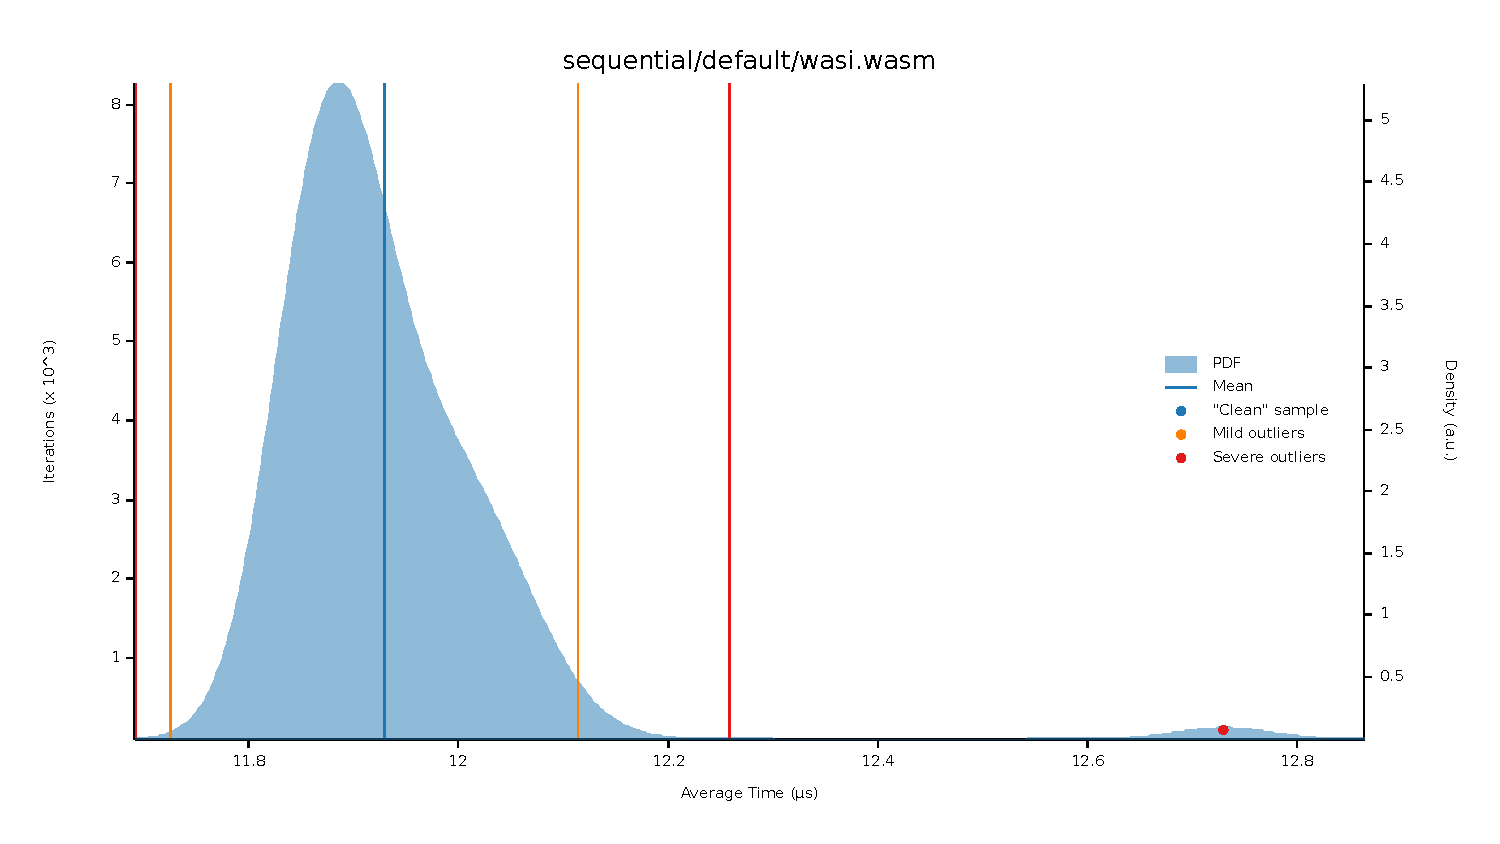
\includegraphics[width=1\linewidth]{images/benches/t2_medium_sequential_default_wasi.pdf}
    \caption{t2.medium, distribution: average instantiation time of a WASI module with Wasmtime}
    \label{fig:bench:t2-instantiation:wasi}
\end{figure}

\begin{figure}[H]
    \centering
        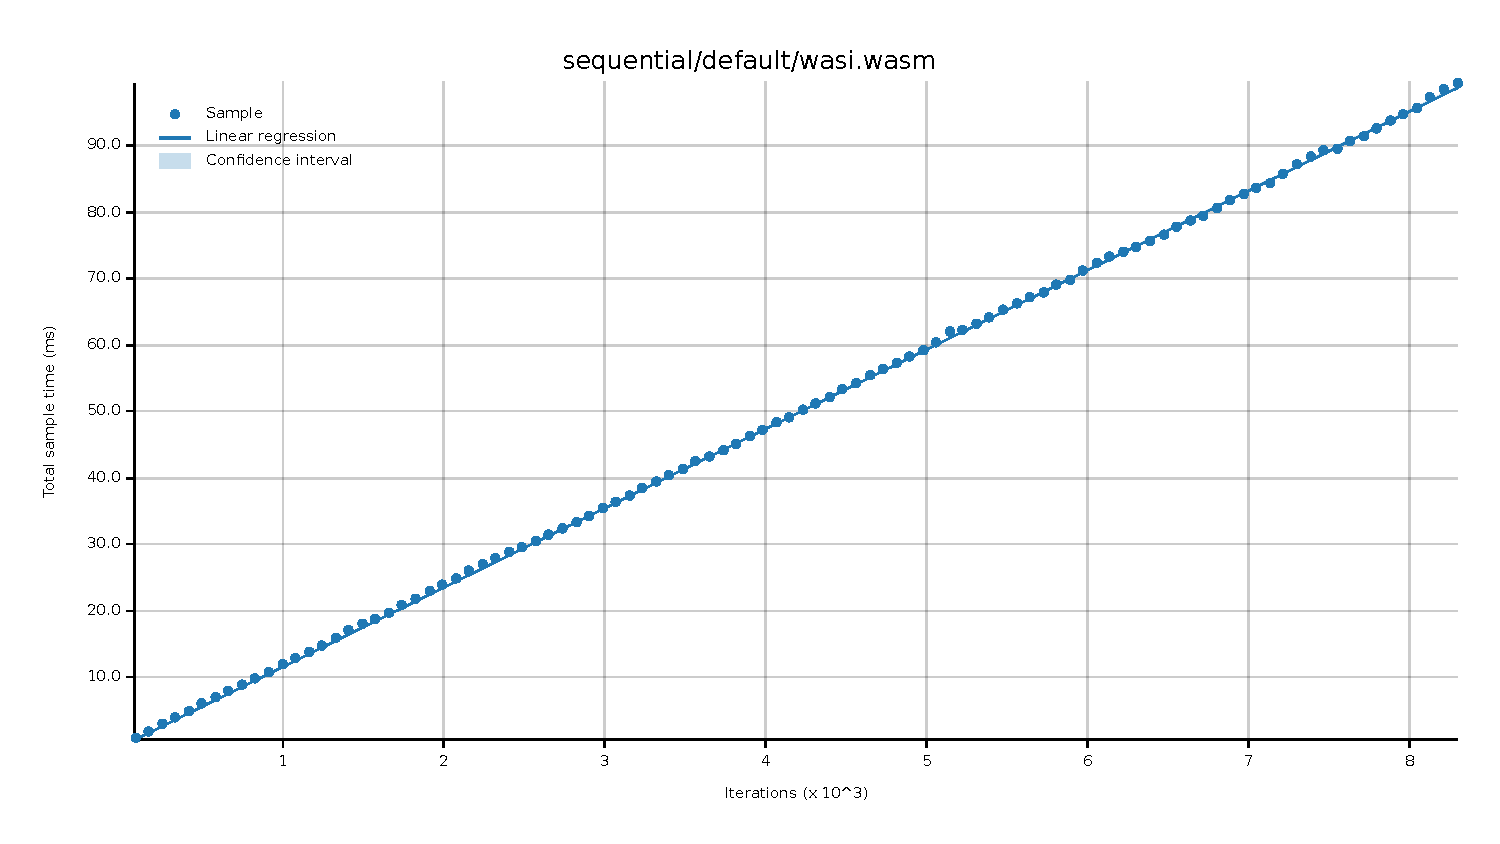
\includegraphics[width=1\linewidth]{images/benches/t2_medium_regression_default_wasi.pdf}
    \caption{t2.medium, linear regression: instantiation of a WASI module with Wasmtime (a smaller distance to the regression line indicates better accuracy)}
    \label{fig:bench:t2-regression-instantiation:wasi}
\end{figure}

\begin{figure}[H]
    \centering
        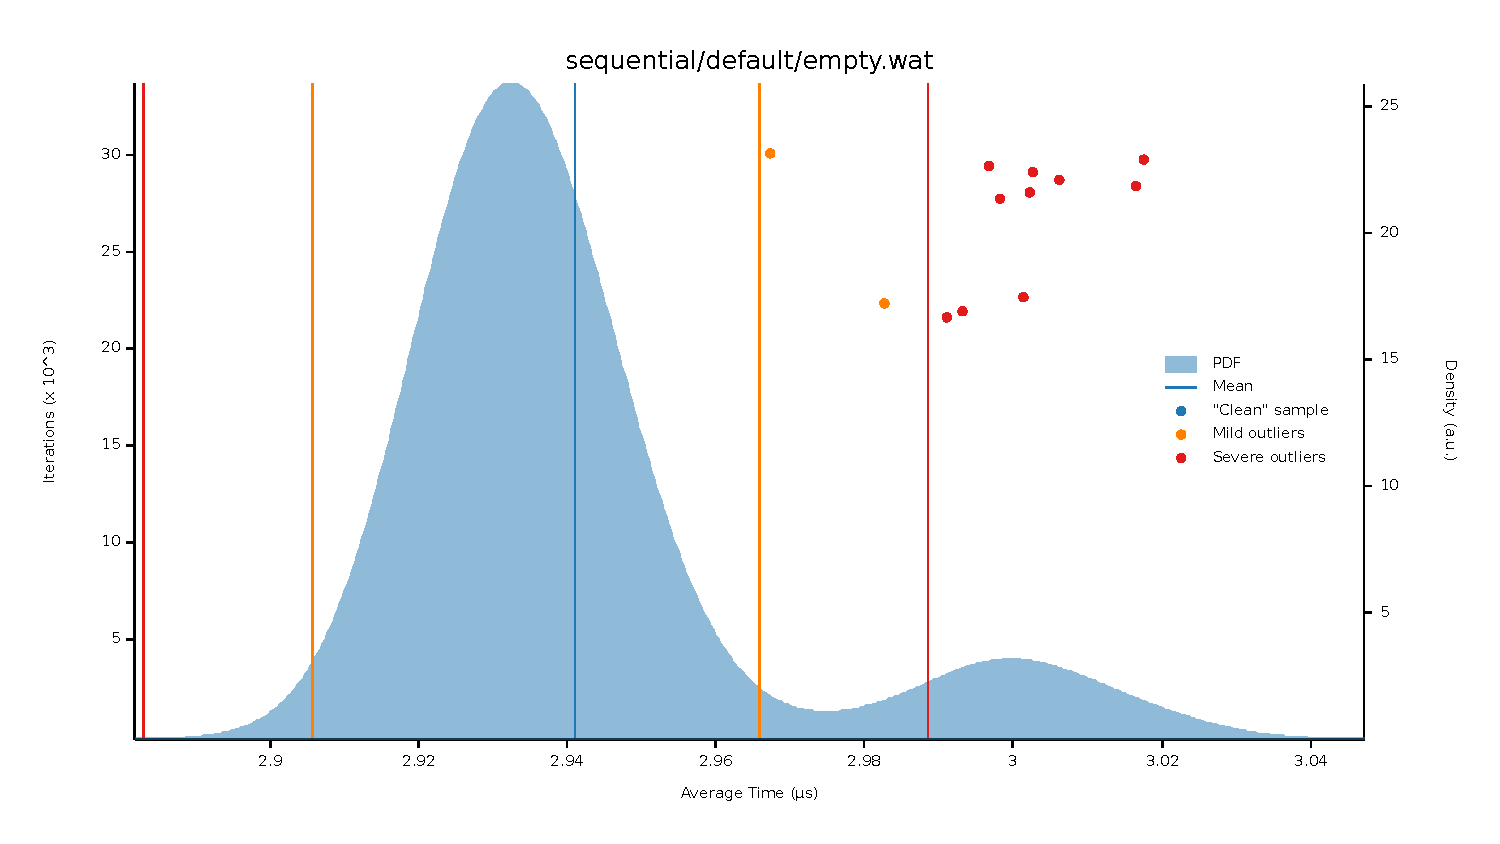
\includegraphics[width=1\linewidth]{images/benches/t2_medium_sequential_default_empty_wasm.pdf}
    \caption{t2.medium, distribution: average instantiation time of an empty Wasm module with Wasmtime}
    \label{fig:bench:instantiation:t2-empty-wasm}
\end{figure}

\begin{figure}[H]
    \centering
        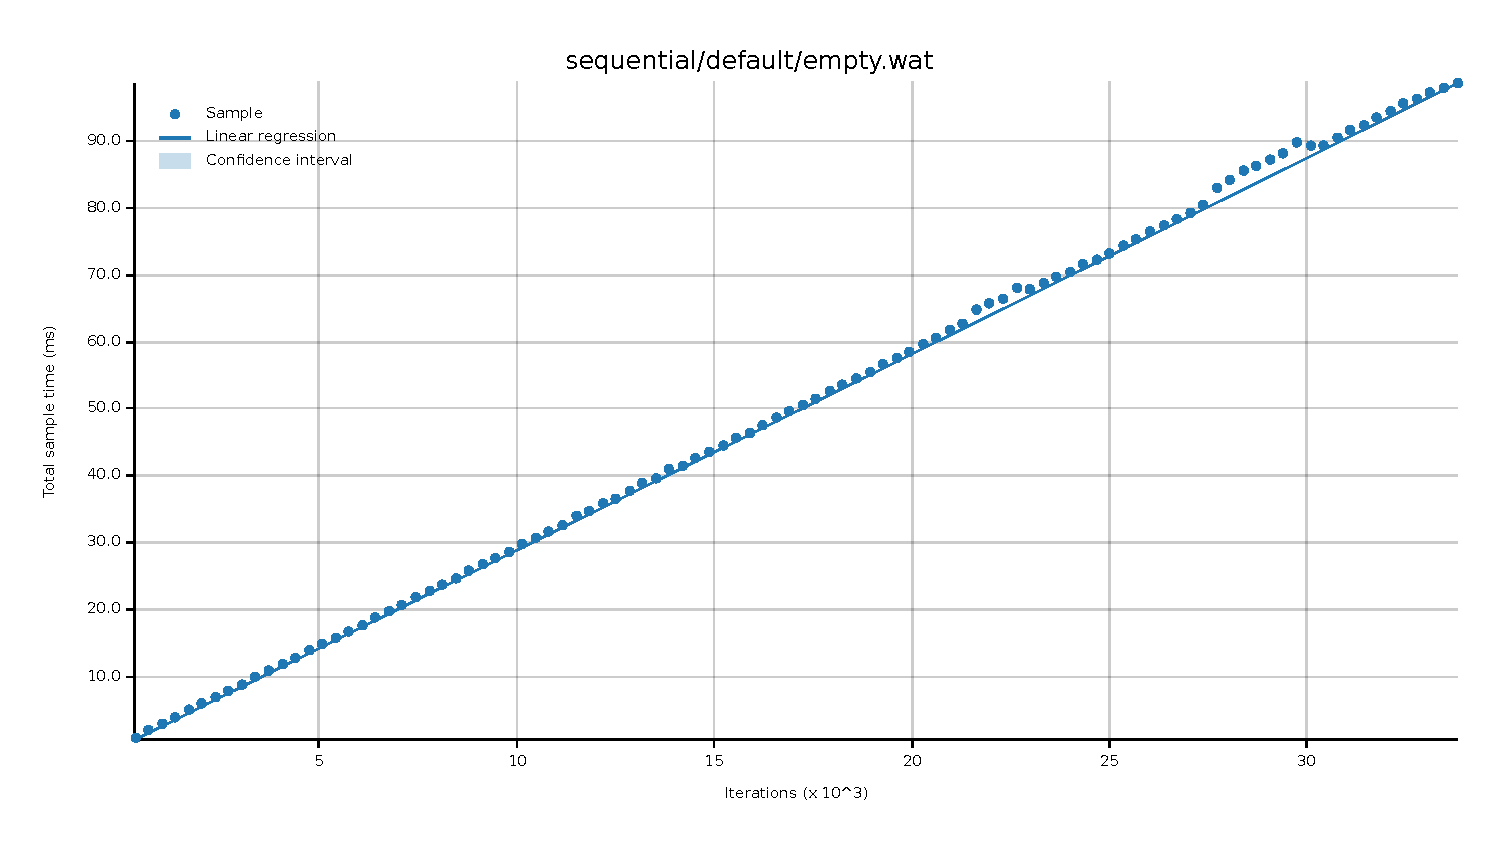
\includegraphics[width=1\linewidth]{images/benches/t2_medium_regression_default_empty.pdf}
    \caption{t2.medium, linear regression: instantiation of an empty Wasm module with Wasmtime (a smaller distance to the regression line indicates better accuracy)}
    \label{fig:bench:instantiation:t2-regression-empty-wasm}
\end{figure}

\begin{figure}[H]
    \centering
        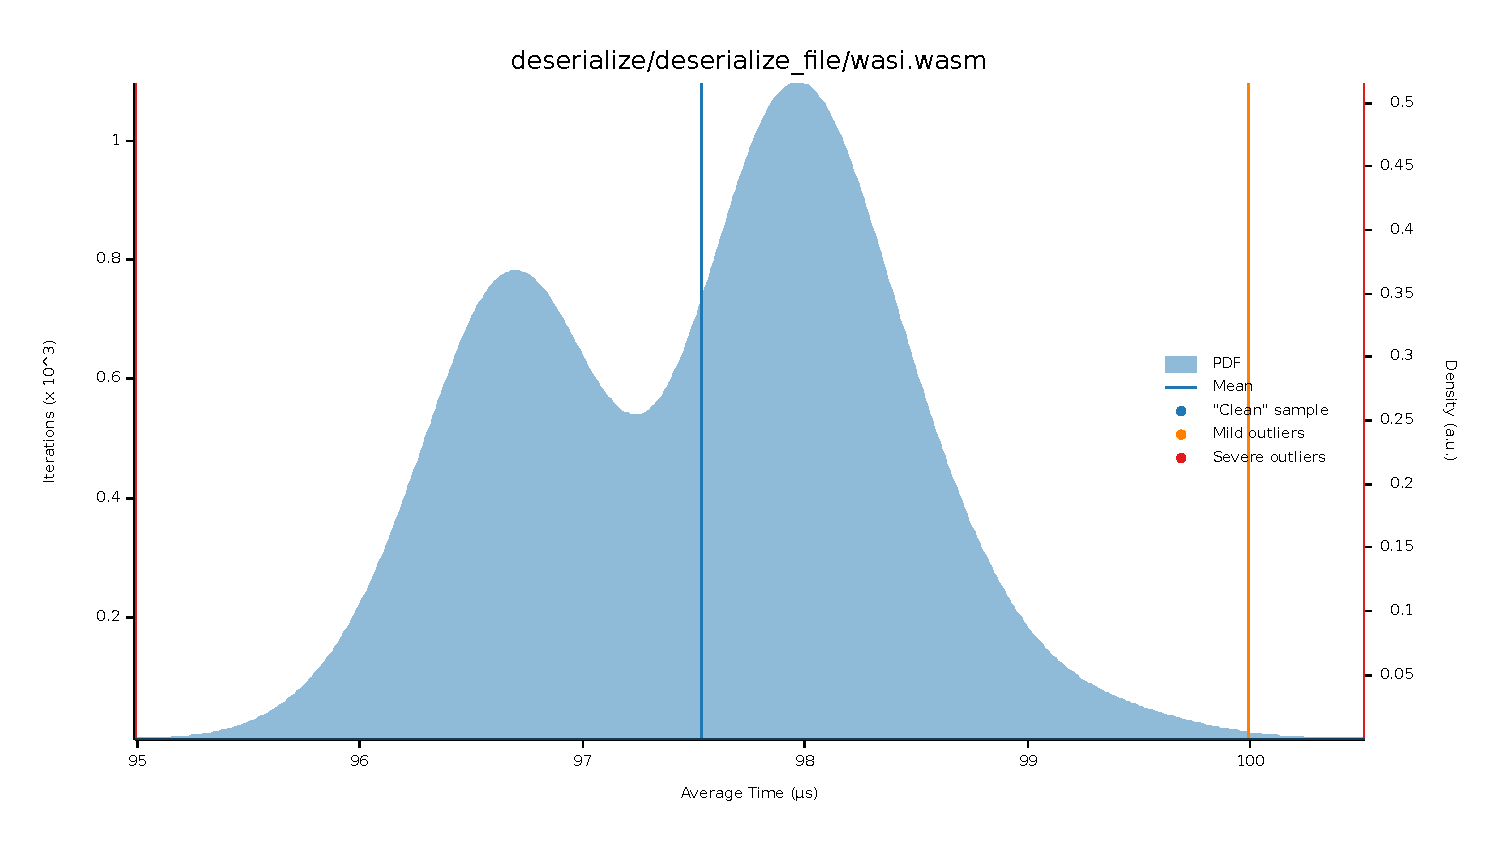
\includegraphics[width=1\linewidth]{images/benches/t2_medium_deserialize_file_wasi.pdf}
    \caption{t2.medium, distribution: average deserialization and instantiation time of a WASI module with Wasmtime}
    \label{fig:bench:instantiation:t2-deserialize-wasi-wasm}
\end{figure}

\begin{figure}[H]
    \centering
        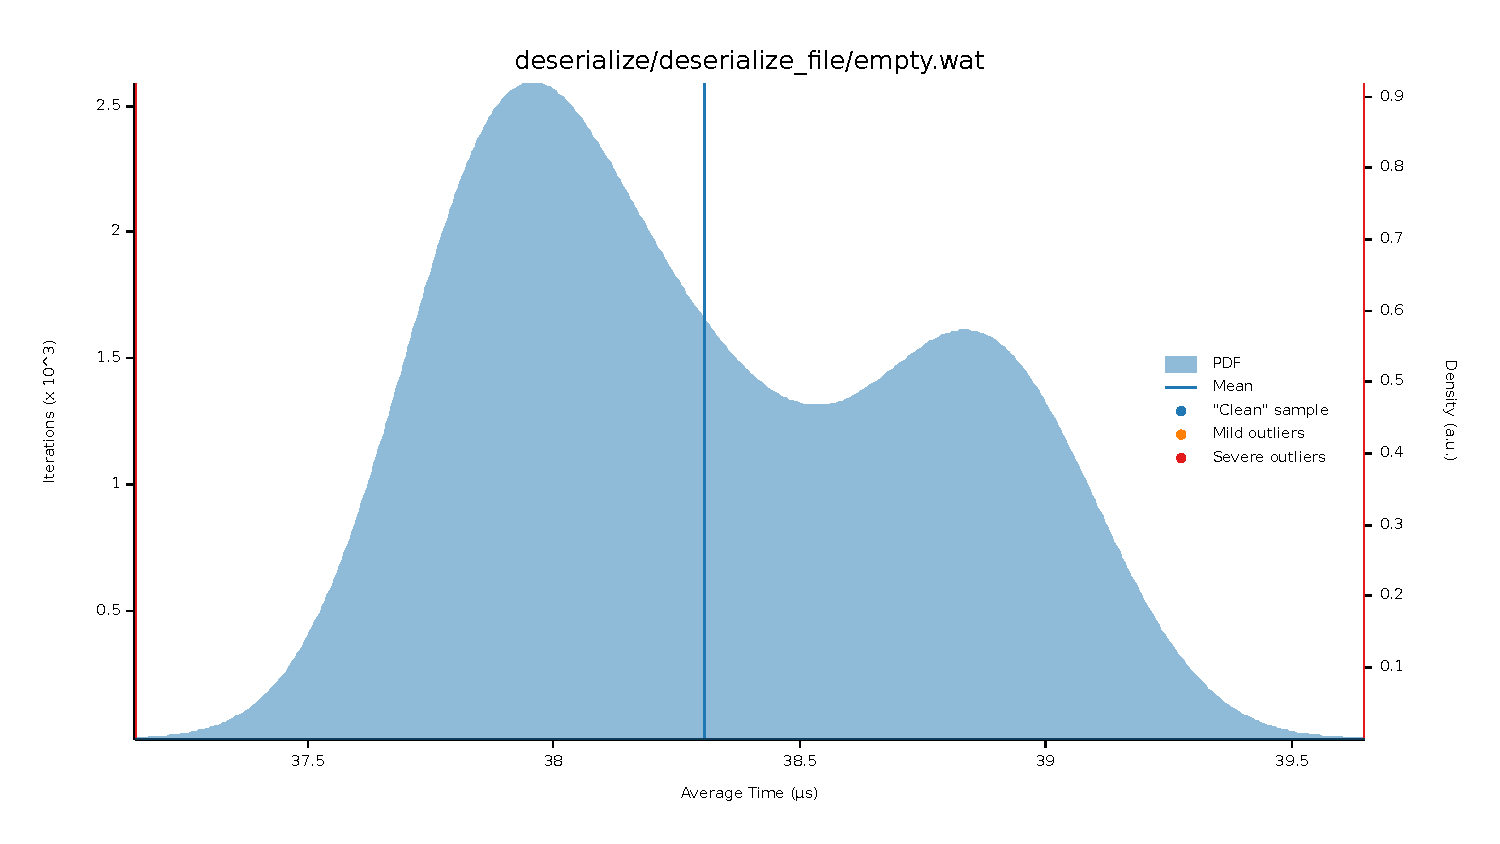
\includegraphics[width=1\linewidth]{images/benches/t2_medium_deserialize_file_empty.pdf}
    \caption{t2.medium, distribution: average deserialization and instantiation time of an empty Wasm module with Wasmtime}
    \label{fig:bench:instantiation:t2-deserialize-empty-wasm}
\end{figure}

\begin{figure}[H]
    \centering
        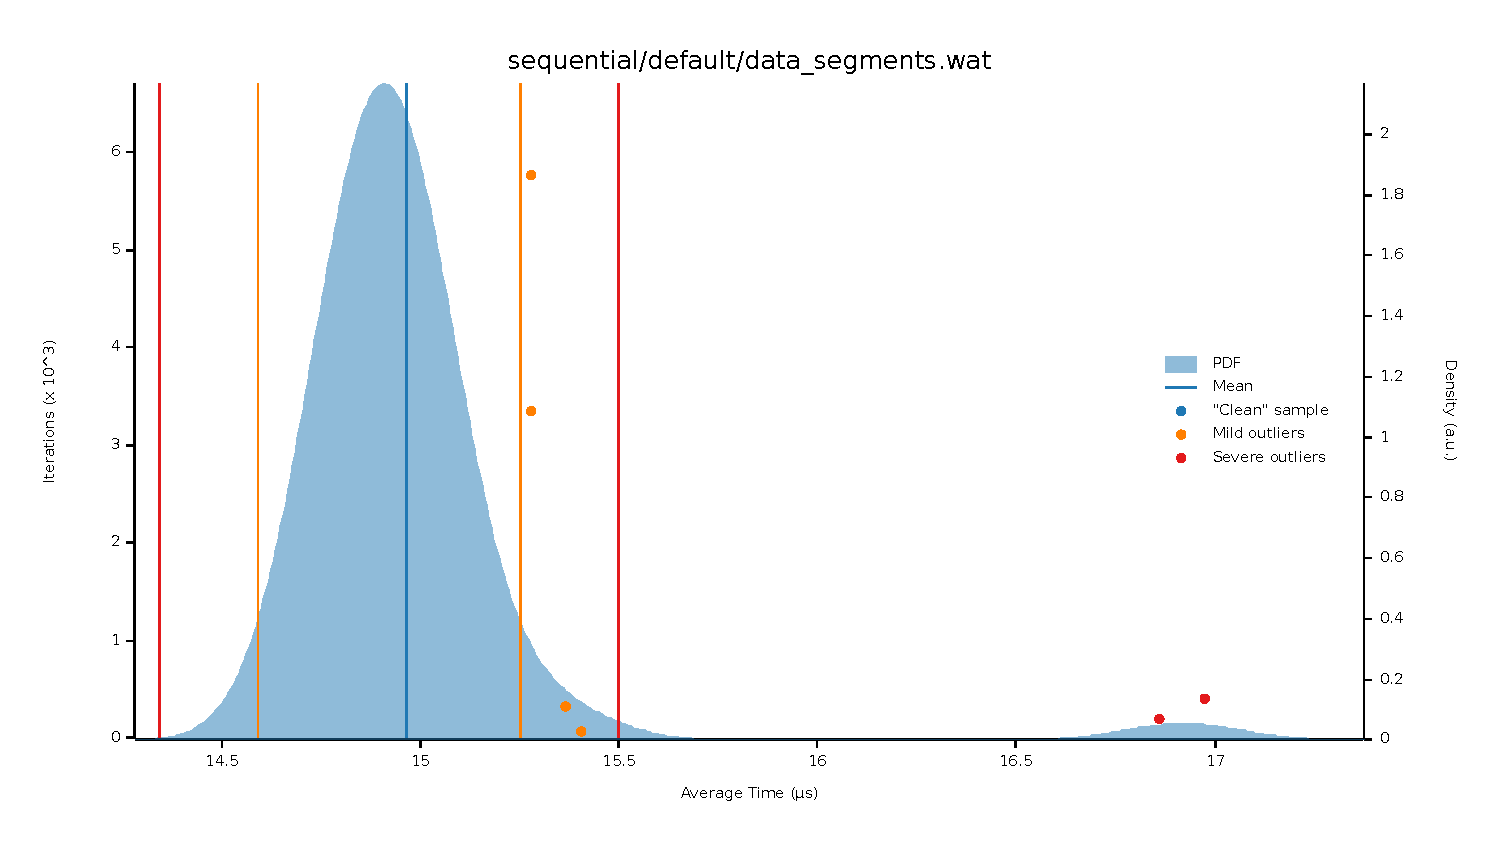
\includegraphics[width=1\linewidth]{images/benches/m1pro_data_segments.pdf}
    \caption{M1 Pro CPU, distribution: average instantiation time of a WASI module containing a large data segment with Wasmtime}
    \label{fig:bench:m1-instantiation:data-segment}
\end{figure}

\begin{figure}[H]
    \centering
        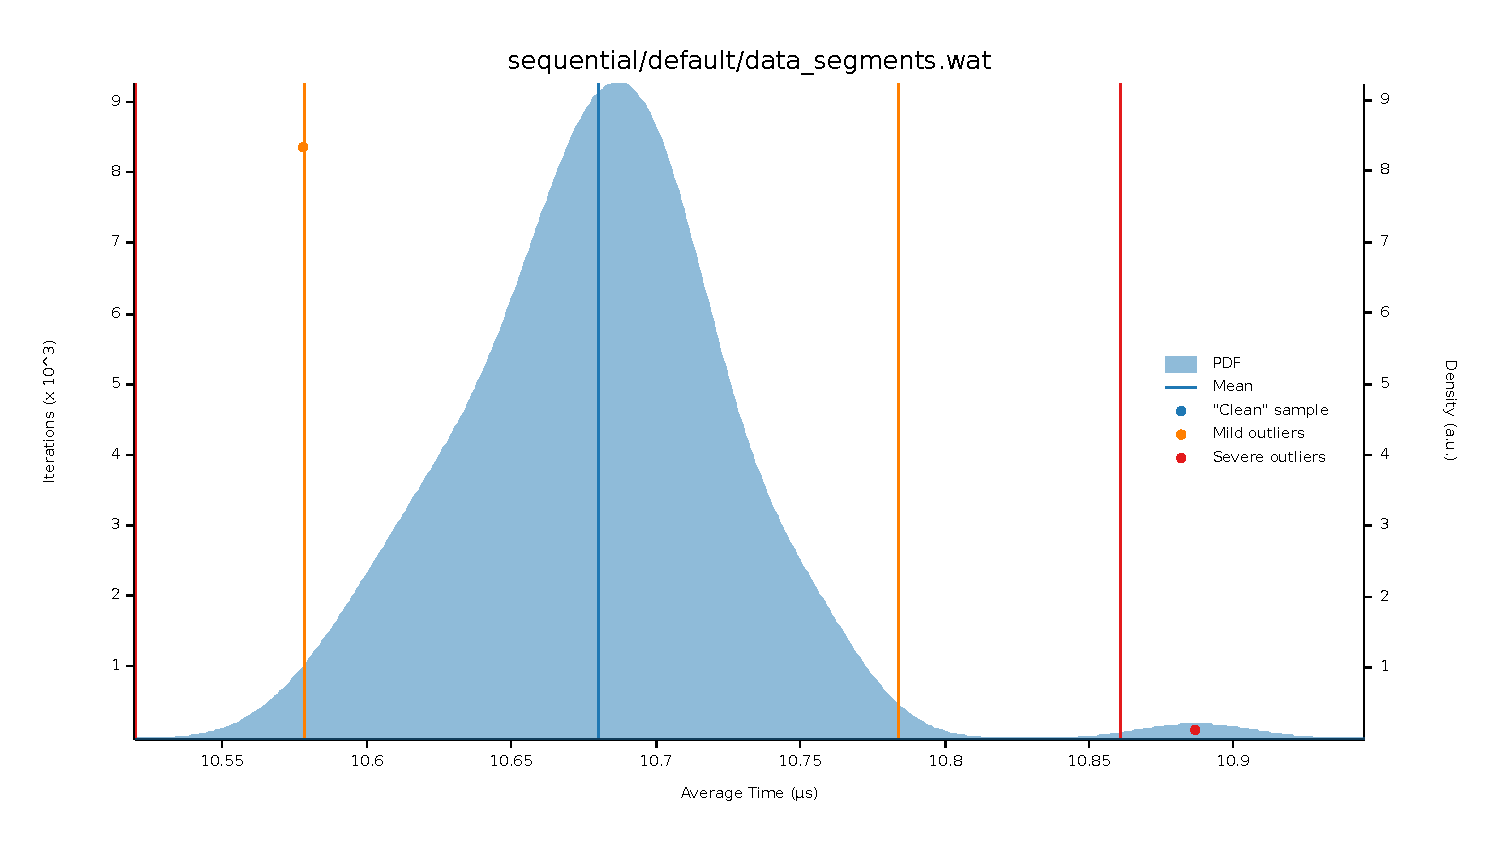
\includegraphics[width=1\linewidth]{images/benches/t2_medium_data_segments.pdf}
    \caption{t2.medium, distribution: average instantiation time of a WASI module containing a large data segment with Wasmtime}
    \label{fig:bench:t2-instantiation:data-segment}
\end{figure}
\newpage

\section*{Serverless Platform Evaluation Curl Results}

\begin{lstlisting}
# process_time is TTFB - (time_connect - time_namelookup)
# Time To First Byte (TTFB) alias time_starttransfer

# Rust, Fibonacci 32, Fastly Compute@Edge
time_namelookup: 0.000820s
time_connect: 0.001207s
time_appconnect: 0.086769s
time_pretransfer: 0.086885s
time_redirect: 0.000000s
time_starttransfer: 0.094141s
----------
time_total: 0.094196s
process_time: 0.094141 - (0.001207 - 0.000820) = 0.093754s = 93,75ms

# Go, Fibonacci 32, Fastly Compute@Edge
time_namelookup: 0.000813s
time_connect: 0.001200s
time_appconnect: 0.086132s
time_pretransfer: 0.086228s
time_redirect: 0.000000s
time_starttransfer: 0.095094s
----------
time_total: 0.095142s
process_time: 0.095094 - (0.001200 - 0.000813) = 0.094707s = 94,71ms

# JavaScript, Fibonacci 32, Fastly Compute@Edge
time_namelookup: 0.000821s
time_connect: 0.001200s
time_appconnect: 0.085285s
time_pretransfer: 0.085414s
time_redirect: 0.000000s
time_starttransfer: 0.131382s
----------
time_total: 0.131449s
process_time: 0.131382 - (0.001200 - 0.000821) = 0.131003s = 131ms

# JavaScript, Fibonacci 32, Cloudflare Workers
time_namelookup: 0.000758s
time_connect: 0.001870s
time_appconnect: 0.090422s
time_pretransfer: 0.090531s
time_redirect: 0.000000s
time_starttransfer: 0.114824s
----------
time_total: 0.114920s
process_time: 0.114824 - (0.001870 - 0.000758) = 0.113712s = 113ms

# JavaScript, Fibonacci 32, AWS Lambda, COLD START
time_namelookup:    0.004100s
time_connect:       0.005111s
time_appconnect:    0.085122s
time_pretransfer:   0.085169s
time_redirect:      0.000000s
time_starttransfer: 0.504372s
------------------------------------------
time_total:         0.504477s
process_time: 0.504372 - (0.005111 - 0.004100) = 0.503361s = 503ms

# JavaScript, Fibonacci 32, AWS Lambda, WARM START
time_namelookup: 0.000788s
time_connect: 0.001157s
time_appconnect: 0.085358s
time_pretransfer: 0.085399s
time_redirect: 0.000000s
time_starttransfer: 0.121778s
----------
time_total: 0.121837s
process_time: 0.121778 - (0.001157 - 0.000788) = 0.121409s = 121ms

# Rust, Blake3 100.000 iterations, Fastly Compute@Edge
time_namelookup:    0.024949s
time_connect:       0.026306s
time_appconnect:    0.106740s
time_pretransfer:   0.106850s
time_redirect:      0.000000s
time_starttransfer: 0.135364s
------------------------------------------
time_total:         0.135422s
process_time: 0.135364 - (0.026306 - 0.024949) = 0.133007s = 133ms
\end{lstlisting}